\section{Introduction}

Multi-objective Optimization Problems (MOPs)~\cite{miettinen1999nonlinear} are problems composed by two or more functions which must be simultaneously optimized by the same set of parameters. This composition is characterized by a set of conflicting objective functions resulting in a set of optimal compromise solutions. 

These $m$ multiple objective functions must be optimized simultaneously:

\begin{align}\label{min_problem}
\text{minimize} f(x) = (f_1(x), ..., f_{m}(x)), \text{ with $x \in \mathbb{R}^{D}$},
\end{align}

where $m$ is the number of objective functions and $\mathbb{R}^m$ is the objective function space. $x \in \mathbb{R}^{D} = \{x_1, x_2, ..., x_D\}$ is a D-dimensional vector and it represents a candidate solution with ${D}$ variables, $f: \mathbb{R}^{D} \rightarrow \mathbb{R}^{m}$ is a vector of objective functions.% and $\Omega$ is the feasible decision space. $\Omega$ is defined as:

%\begin{align}
%\Omega =\{x \text{ in } \mathbb{R}^{n_v} | g_i(x) \leq 0 \text{ } \forall_i \text{ and } h_i(x) = 0 \text{ } \forall_j \},
%\end{align}
Objectives often conflict with each other therefore no point in $\Omega$ minimizes all the objectives at the same time. Consequently, the goal of MOP solvers is to find the best trade-off that balances the different objectives in an optimal way.

Given two feasible solutions vectors $u, v$ in $\Omega$, $u$  Pareto-dominates $v$, denoted by $f(u) \prec f(v)$, if and only if $f_k(u) \leq f_k(v), \forall_k \in \{1,..., m\}$ and $ f(u) \neq f(v)$. 

A solution $x \in \mathbb{R}^{D}$ is considered Pareto-Optimal if there exists no other solution $y \in \mathbb{R}^{D}$ such that $f(y) \succ f(x)$, i.e., if $x$ is non-dominated in the feasible decision space. A point is called non-dominated if no other point dominates it. That is, no single solution provides a better trade-off in all objectives.

The set of all Pareto-optimal solutions is known as the Pareto-Optimal Set (PS), while the image of this set is referred to as the Pareto-optimal Front (PF).\\

\begin{equation}
PS = \{x \in \Omega | \nexists y \in \Omega : f(y) \succ f(x^*)  \},
\end{equation}

\begin{equation}
PF = \{f(x) | x \in PS \}.
\end{equation}

Multi-objective evolutionary algorithms (MOEAs) are characterized by their ability to find good approximations the PF of a MOP in a single run~\cite{zhou2011multiobjective}.Over the last two decades, many different search techniques were proposed for improving the effectiveness of multi-objective algorithms. Among them, three are the major paradigms: Pareto domination-based approaches~\cite{deb2002fast},~\cite{zitzler2001spea2}, the indicator-based approaches~\cite{beume2007sms},~\cite{zitzler2004indicator}, and the decomposition-based approaches~\cite{li2009multiobjective},~\cite{zhang2007moea}. 


Multi-objective Evolutionary Algorithm based on Decomposition, MOEA/D~\cite{zhang2007moea}, represents a class of population-based meta-heuristics for solving Multi Objective Problems~\cite{trivedi2017survey}. In this search paradigm, the original multi-objective problem is decomposed into simpler, single-objective subproblems by means of scalarizations, see Figure~\ref{fig1}.
However, it may waste functions evaluations searching in directions that do not present Pareto-optimal solutions~\cite{bezerra2015comparing}. As in the example of Figure~\ref{fig2}, some vector represent "empty regions" of the PF.
\begin{figure}[h]
	\centering
	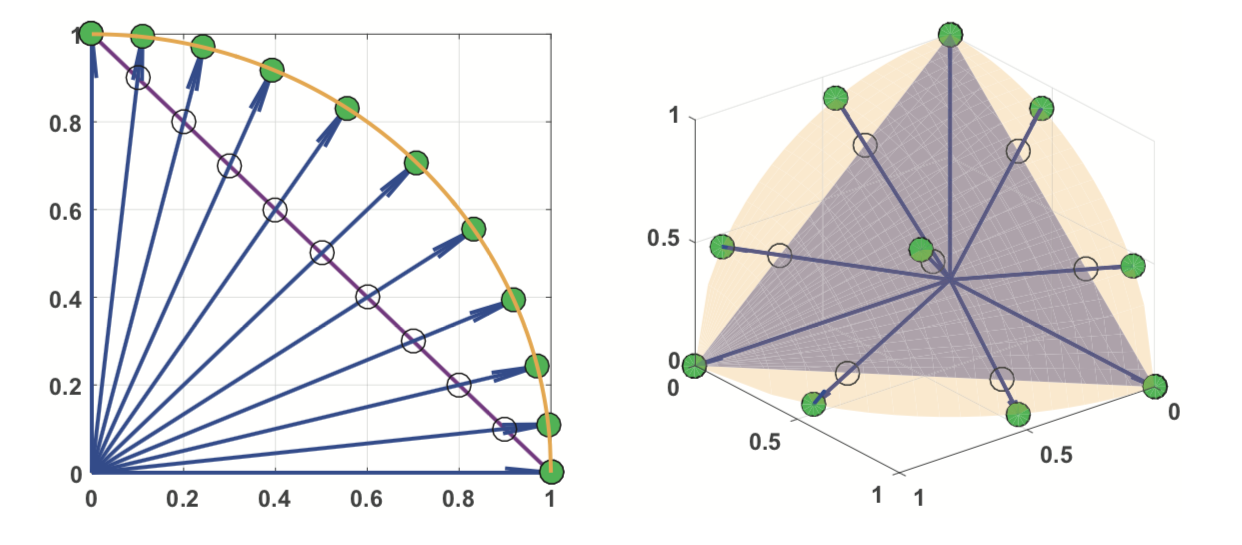
\includegraphics[width=0.55\textwidth]{img/decomp2.png}
	\caption{A decomposition strategy generates weight vectors that defines the subproblems. Figure from~\cite{chugh2017handling}.}
	\label{fig1}
\end{figure}

\begin{figure}[h]
	\centering
	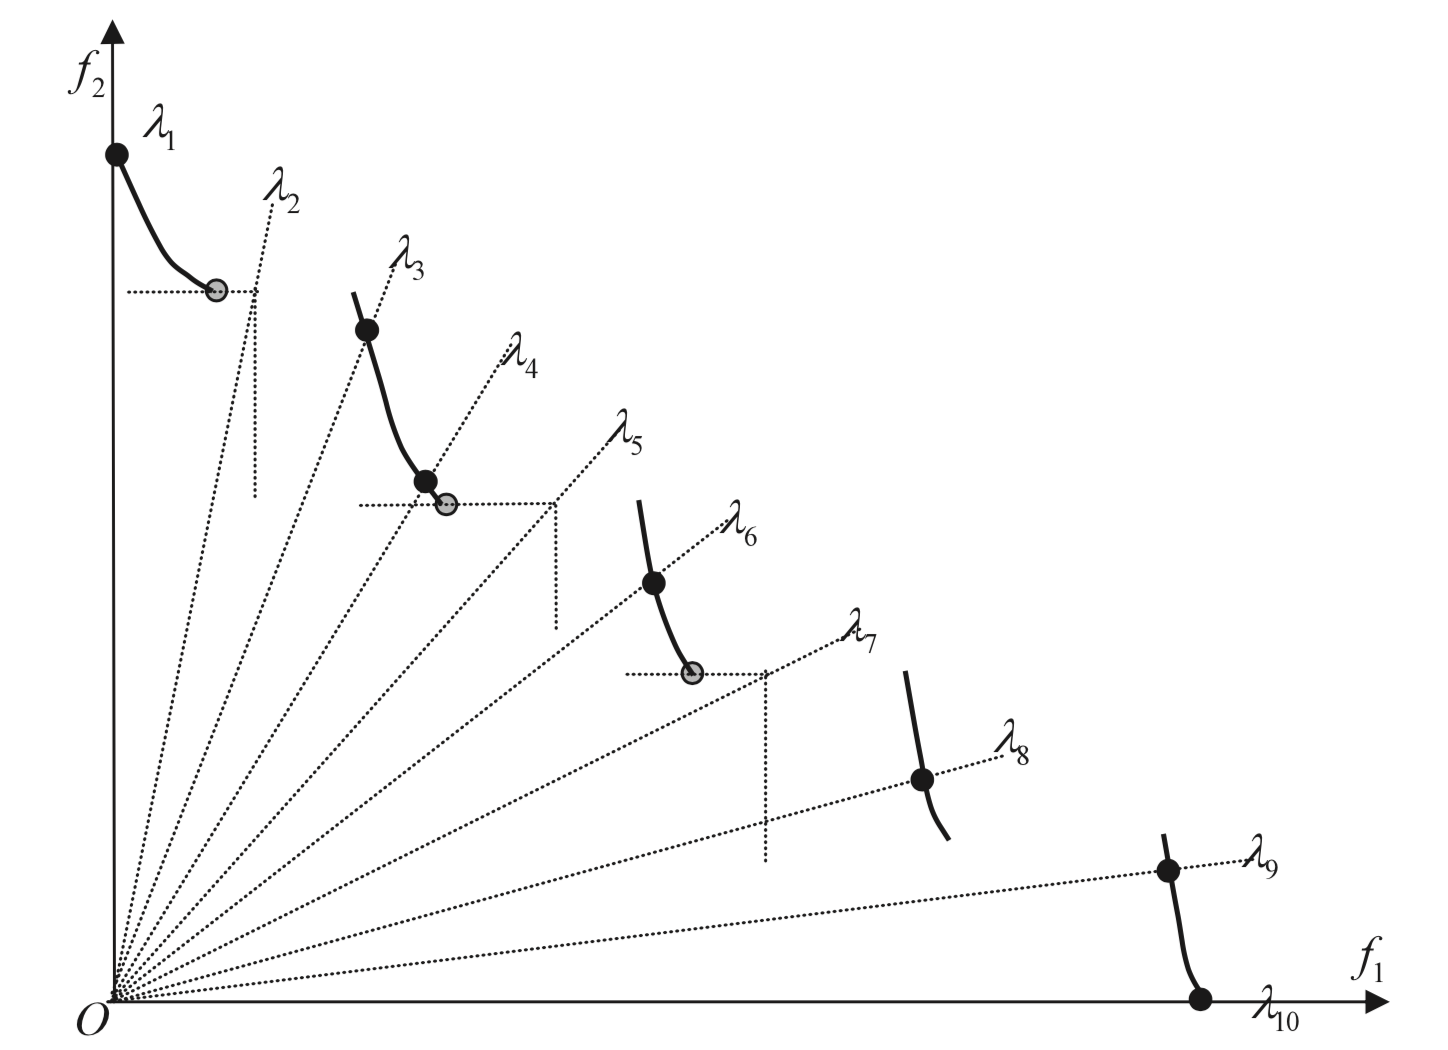
\includegraphics[width=0.43\textwidth]{img/harder_problems}
	\caption{Distribution of optimal solutions of subproblems with uniform weight vectors on ZDT3. Figure from~\cite{li2015use}.}
	\label{fig2}
\end{figure}


\begin{figure}[h]
	\centering
	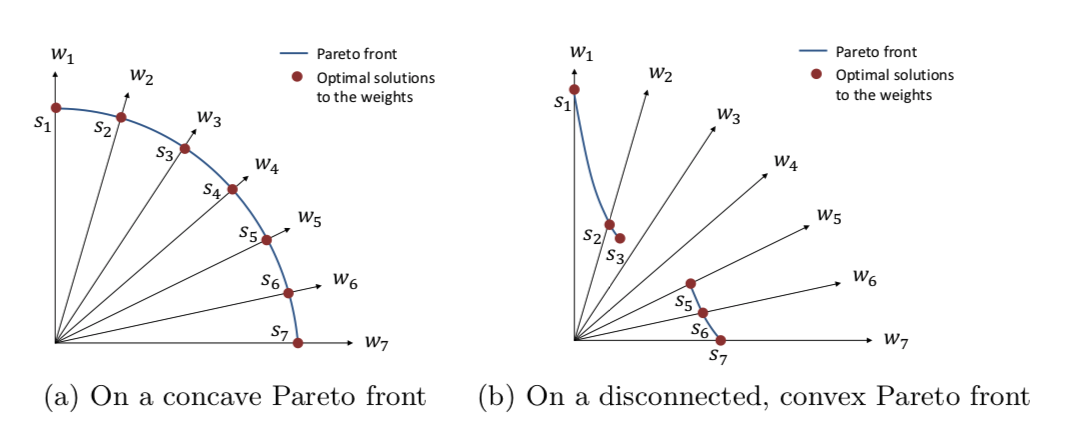
\includegraphics[width=0.53\textwidth]{img/harder_problems2}
	\caption{An example that uniformly distributed weights may lead to different distributions of optimal solutions. (a) Solutions $s_1$ to $s_7$ are the optimal solutions of weights $w_1$ to $w_7$, respectively. (b) Solutions $s_1$,$s_2$,$s_3$,$s_6$ and $s_7$ are the optimal solutions of $w_1$,$w_2$,$w_3$,$w_6$ and $w_7$, respectively, while solution $s_5$ is the optimal solution of $w_4$ and $w_5$.Figure from~\cite{li2017weights}}
	\label{fig3}
\end{figure}

In the original MOEA/D~\cite{zhang2007moea}, all the subproblems have the same amount of computational resource (number of iteractions). It has been observed, as one can expect that some parts of the theoretical Pareto Front PF, in an MOP can be more difficult to approximate than others, Figure~\ref{fig3},~\cite{zhang2009performance}~\cite{zhou2016all}~\cite{kang2018collaborative}.

%It represents a class of population-based meta-heuristics for solving MOPs. Many other algorithms exists as NSGA-2(3), MOEA/Ds, IBEA, SPEA2, DEMO.

This difficulties on approximating the PF may lead to a unbalanced exploration of the search space. One of the reasons is that, given to this dissimilar conditions, the number of iteractions needed will possibly not be the same. 

 To reduce this computational cost, the allocation of resources may be better distributed among different sub-problems according to their difficulties. One way to address this problem is to adjust the behavior of the algorithm in an on-line manner to suit the problem in question~\cite{hinterding1997adaptation},~\cite{de2007parameter},~\cite{meyer2007self},~\cite{zhang2009performance},~\cite{kramer2010evolutionary},~\cite{zhang2012survey}~\cite{cai2015external}. All algorithmic components can be tunned adaptively and often feedback information is needed for these adaptation strategies. 

Another way, is to allocate different amounts of resources to the subproblems based on some priority function. In a few recent works recently proposed, a utility function is being used to distribute the resources given priorities to subproblems that contribute more to the algorithm's search.  In the works of Zhang et al.~\cite{zhang2009performance} and Zhou et al.~\cite{zhou2016all} the a utility function was proposed aiming to prioritize solutions based on a historical convergence information during different generations. Another approach was implemented in~\cite{kang2018collaborative}, where the utility function was based on the presence of a solution from the main population on a secondary population.

%The main contributions of this paper can be summarized as follows:

%\begin{itemize}
%	\item blablabla
%	\item blebleble
%	\item bliblibli
%\end{itemize}

This work is divided in sections and subsections according to this and that.

